\newcommand{\lc}{LC}
\newcommand{\ta}{TA}
\newcommand{\smc}{SMC}
\newcommand{\kcore}{k_{core}}
\newcommand{\kmesh}{k_{mesh}}
\newcommand{\kram}{k_{ram}}

\lstset{
language=C,
numbers=left,
numberstyle=\footnotesize,
frame=single}

\lstset{deletekeywords={bool,int}}
\lstset{morekeywords={foreach,in}}

\lstset{classoffset=1, morekeywords={ZERO,ONE,LOCAL\_MANY,GLOBAL,FORWARDED},keywordstyle=\color{Red},
        classoffset=2, morekeywords={pointer,bool,int,Val,Ref,ThreadID,Thread,Set},keywordstyle=\color{OliveGreen}, %Types
        classoffset=0}% restore default


\chapter{\MMSCC: A Coherent and Managed Runtime for ML on the SCC}
\label{chap:aneris}

In this chapter, we describe \MMSCC, an extension of \MM that provides a
coherent address space on the SCC, optimizing for the SCC's memory hierarchy.
We begin with a \emph{local collector}\footnote{Other terms have been used in
the literature to indicate similar heap designs, notably private nursery, local
heap collector, thread-local or thread-specific heap, and on-the-fly
collection.} (\lc) design~\cite{} that partitions the heap into local heaps on
each core and a shared heap for cross-core communication. However, we observe
that the cost of memory barriers utilized in preserving the heap invariants
have significant costs. To eliminitate theses costs, we propose a new GC design
(\ta) that utilizes the ample concurrency offered by our programming model
combined with a dynamic shape analysis to eliminate some of the GC overheads.
This naturally leads to a GC design that focuses on
\emph{procrastination}~\cite{mmgc}, delaying writes that would necessitate
establishing forwarding pointers until a GC, where there is no longer a need
for such pointers. The GC leverages the mostly functional nature of ACML
programs and a new object property called \emph{cleanliness}, which enables a
broad class of objects to be moved from a local to a shared heap without
requiring a full traversal of the local heap to fix existing references;
cleanliness enables an important optimization that achieves the effect of
procrastination without actually having to initiate a thread stall. Our final
design (\smc) integrates SCC's support for software-managed cache coherence
into the extant memory barriers to improve the design further.

We begin by discussing in detail the architecture and programming model of the
SCC, which serves as our prototype non cache coherent architecture. However,
the use of SCC by no means restricts the applicability of our ideas to other
scalable manycore architectures~\cite{mmgc}.

\section{The Intel Single-chip Cloud Computer}

\begin{figure}
\begin{center}
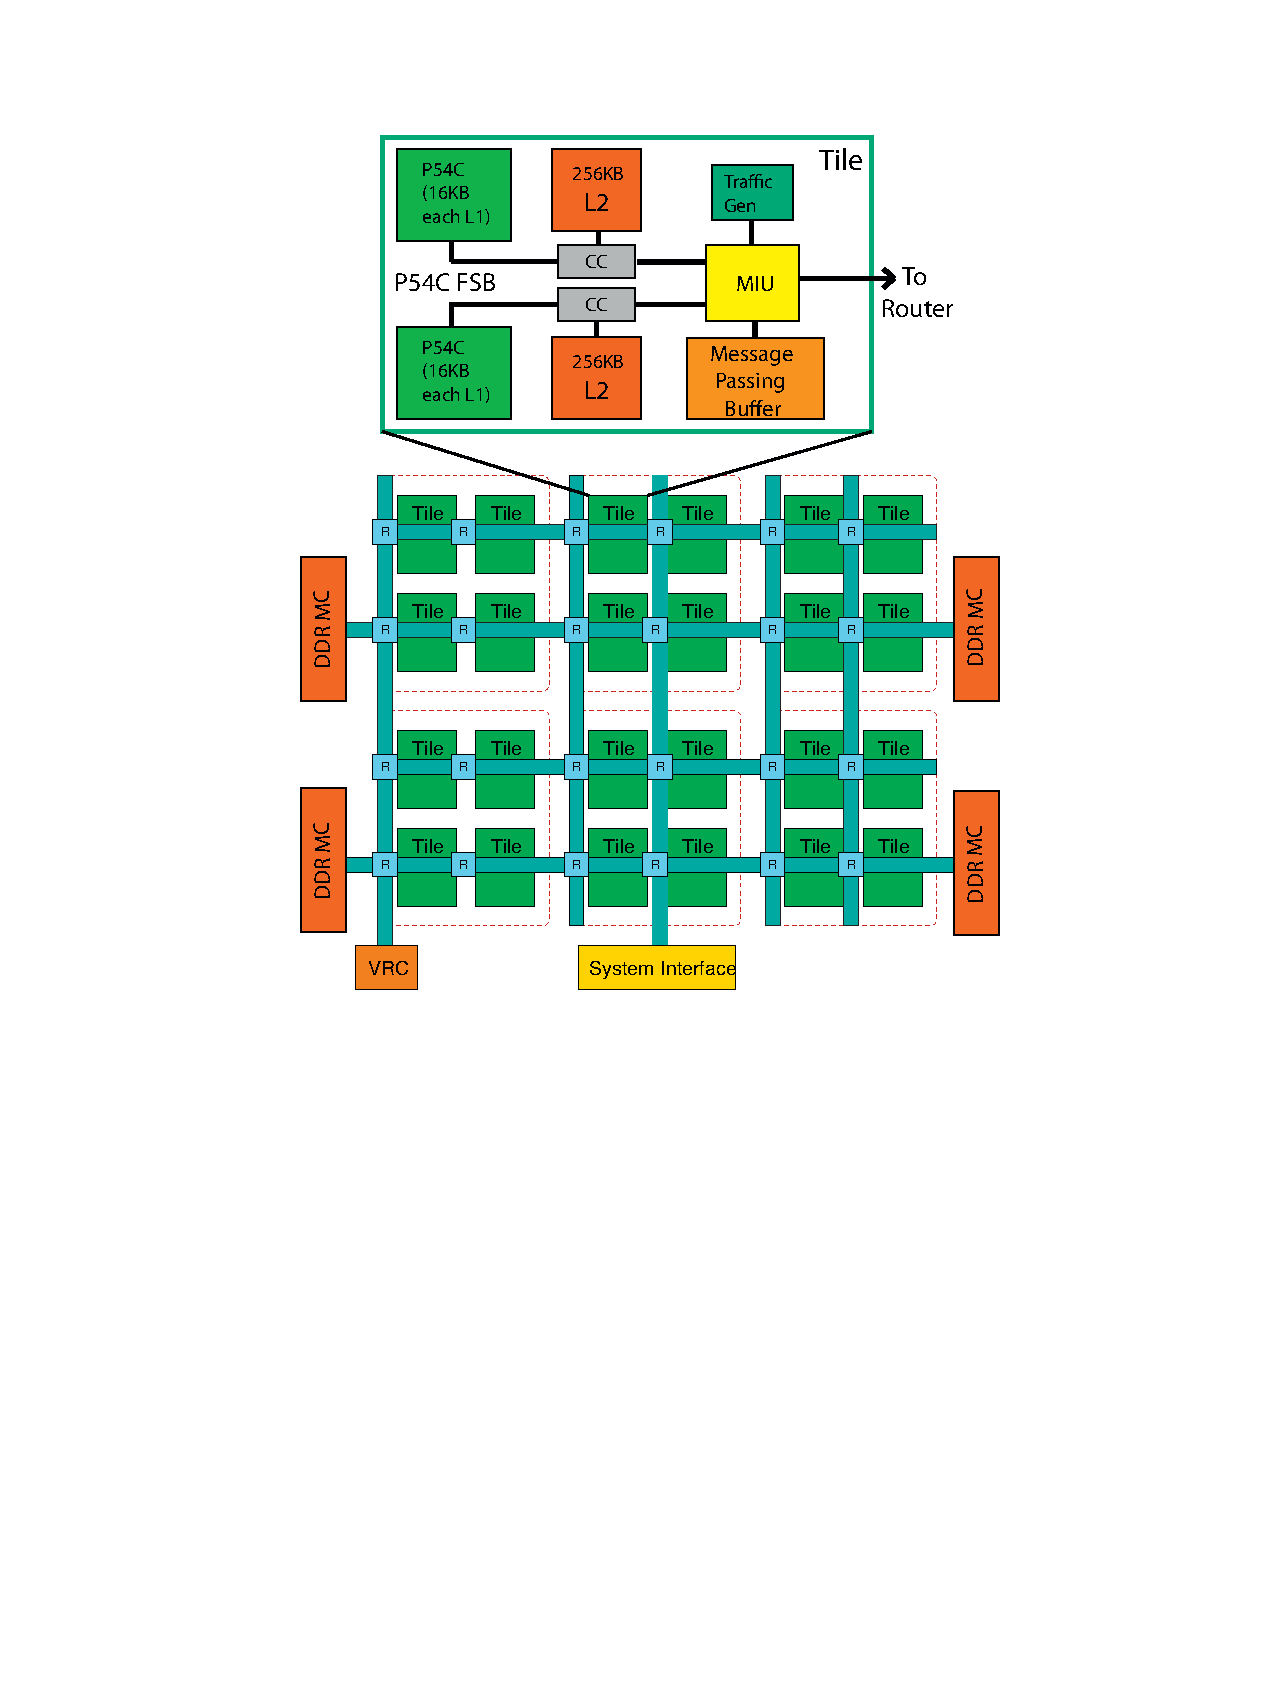
\includegraphics{Figures/SCC.pdf}
\end{center}
\caption{The architecture of the Intel SCC processor}
\label{fig:scc}
\end{figure}

Intel SCC~\cite{Mattson2010} (Figure~\ref{fig:scc}) is a many-core processor
with 48 P54C cores on a single chip, grouped as 24 tiles, organized in a 4
$\times$ 6 mesh network with a bisection bandwidth of 256 Gb/s. The most
interesting aspect of the SCC architecure is the complete lack of cache
coherence between the cores, and the presence of fast on-die message-passing
network interface. The 24 tiles on the chip are divinded into 4 quadrants, and
each quadrant is connected to a DDR3 memory controller. Each core has 16KB of
private L1 instruction and data caches, and 256 KB of L2 cache shared with the
other core on the same tile.

In addition, each tile has a 16KB message-passing buffer (MPB) used for
message-passing between the cores. The message passing buffers are the only
caches that are accessible across all of the cores. The data used in on-chip
communication is read from MPB, cached in L1 cache, but bypasses the L2 cache.
The cache uses no-allocate policy on writes, and L1 cache incorporates a
write-combine buffer. According to the processor
specifications~\cite{Mattson2010}, the read latencies in this architecure are:
\begin{mathpar}
\begin{array}{rcl}
\textrm{LocalMPB} & = & 45~\kcore + 8~\kmesh \\
\textrm{RemoteMPB} & = & 45~\kcore + 4*n*2~\kmesh \\
\textrm{DRAM} & = & 40~\kcore + 4*n*2~\kmesh + 46~\kram
\end{array}
\end{mathpar}

\noindent where $\kcore$, $\kmesh$ and $\kram$ are the cycles of core, mesh
network and memory respectively. In our experimental setup, where 6 tiles share
a memory controller, the number of hops n to the memory controller could be $0
< n \le 8$. Hence, the DRAM accesses are far more expensive than the MPBs. Each
core additionally has a test and set register that is accessible from all other
cores. The SCC uses 32-bit Pentium cores. A programmable, software-managed
Look-Up Table (LUT) provides a means for implementing hybrid private and shared
address spaces in the system.

\subsection{Software System}

From the programmer's point of view, SCC resembles a cluster of nodes, with
portions of memory shared between the cores. Each core runs a linux kernel
image, and does not share any operating system services with the other cores.
Since SCC does not provide harware cache coherence, it provides software
support for managing coherence. First, SCC provides support for tagging a
specific virtual address space as shared across all of the cores. Caching can
also be selectively enabled on this address space; SCC tags this address space
as having message passing buffer type (MPBT).

Data typed as MPBT bypass L2 and go directly to L1. SCC also provides a
special, 1-cycle instruction called \cf{CL1INVMB} that marks all data of type
MPBT as invalid L1 lines. In addition, special 1-cycle instructions are
provided to flush (\cf{INVFLUSH}) and invalidate (\cf{INV}) L1 cache data.
Since the cores use write-combine buffers, a correct flushing procedure should
also flush the write-combine buffers. SCC does not provide primitive support
for this purpose, but write-combine buffers can easily be flushed in software
by perfoming a series of dummy writes to distinct memory locations, which fills
the buffer and flushes any previous writes. Typically, a programmer works with
release consistency in order to utilize cached shared virtual memory. Let us
assume that a core issues a \cf{smcAcquire()} to fetch changes from other cores
and issues \cf{smcRelease()} to publish its updates.

SCC's software stack also includes cross-core message-passing libraries
implemented over the MPBs, including RCCE~\cite{Mattson2010} and
RCKMPI~\cite{Urena2011}. RCCE is optimized for SPMD~\cite{} programming model,
where the program is structured in such a way that the sender and the receiver
ideally arrive at the communication point at the same time. The sender writes
the message to the MPB, while the receiver busy waits (invalidating its cache
every iteration to fetch recent writes), waiting for a special flag value to be
written along with the message. After the sender writes the flag, the receiver
reads the message into its private memory, while the sender busy waits (also
invalidating its cache every iteration). Finally, the receiver writes a
completion flag, which concludes the message transfer.

It is worthwhile pointing out that RCCE uses just the MPBs, while RCKMPI uses
MPBs for small messages (less than 8KB --- the maximum message size that would
fully fit in the MPB) and the DRAM for larger messages. Despite having a higher
bandwidth and lower latency, the synchronization costs involved in transferring
a large multi-part message over the MPB overweighs the benefits.

\section{Local Collector Design}

Splitting a program heap among a set of cores is a useful technique to exploit
available parallelism on scalable multicore platforms: each core can allocate,
collect, and access data locally, moving objects to a global, shared heap only
when they are accessed by threads executing on different cores. This design
allows local heaps to be collected independently, with coordination required
only for global heap collection. In contrast, stop-the-world collectors need a
global synchronization for every collection.

\begin{figure}
\centering
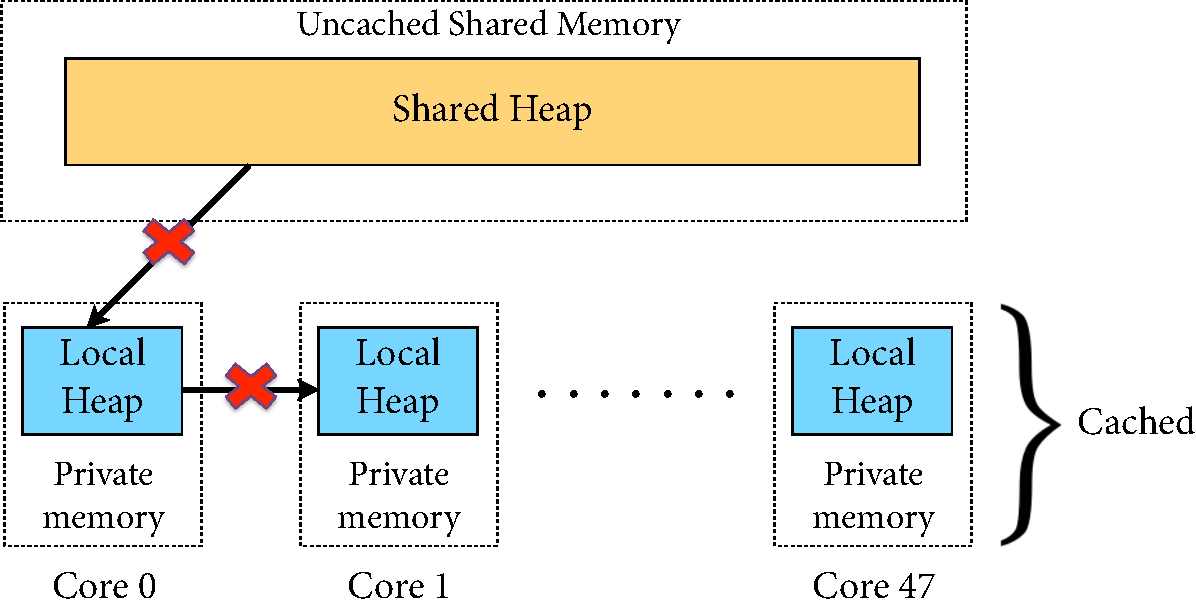
\includegraphics[scale=0.75]{Figures/LocalCollector.pdf}
\caption{Local collector heap organization for the SCC}
\label{fig:lc}
\end{figure}

\subsection{Heap Architecture}

Our local collector design for the SCC is shown in Figure~\ref{fig:lc}. The key
idea here is that the local heaps are allocated in each of the cores
\emph{cached} private memory, into which new objects are allocated by default.
The private heaps are allocated on the memory banks closest to the core to
optimize for the memory hierarchy and reduce mesh congestion. Since the design
allows independent collection of local heaps, the design can scale to hundreds
of cores~\cite{JFP14}, and benefits cache coherent architectures as well. The
shared heap is allocated in the shared memory, and visible to all of the cores.
In order to circumvent the coherence issues, we disable caching on the shared
heap. Hence, every shared memory access goes to the DRAM. The shared heap pages
are interleaved across all of the memory banks to uniformly spread the
requests.

\subsection{Heap Invariants}

In order to ensure that cores cannot directly or indirectly access objects on
other local heaps, which would complicate the ability to perform independent
local heap collection, the following invariants need to be preserved:

\begin{itemize}
\item No pointers are allowed from one core's local heap to another.
\item No pointers are permitted from the shared heap to the local heap.
\end{itemize}

\noindent Both invariants are necessary to perform independent local
collections.  The reason for the first is obvious.  The second invariant
prohibits a local heap from transitively accessing another local heap object
via the shared heap.  In order to preserve these invariants, the mutator
typically executes a \emph{write barrier} on every store operation. The write
barrier ensures that before assigning a local object reference (source) to a
shared heap object (target), the local object along with its transitive object
closure is lifted to the shared heap. We call such writes \emph{exporting
writes} as they export information out of local heaps.  The execution of the
write barrier creates \emph{forwarding pointers} in the original location of
the lifted objects in the local heap. These point to the new locations of the
lifted objects in the shared heap. Since objects can be lifted to the shared
heap on potentially any write, the mutator needs to execute a \emph{read
barrier} on potentially every read. The read barrier checks whether the object
being read is the actual object or a forwarding pointer, and in the latter
case, indirects to the object found on the shared heap.  Forwarding pointers
are eventually eliminated during local collection.

\subsection{Allocation and Collection}

The allocations in the shared heap is performed similar to allocations in the
stop-the-world collector, where each core allocates a page-sized chunk in the
shared heap and performs object allocation by bumping its core-local shared
heap frontier. Allocations in the local heaps do not require any
synchronization. Garbage collection in the local heaps is similar to the
baseline collector, except that it crucially does not require global
synchronization.

Objects are allocated in the shared heap only if they are to be shared between
two or more cores. Objects are automatically lifted to the shared heap because
of exporting writes and spawning a thread on a different core. Apart from
these, all globals are allocated in the shared heap, since globals are visible
to all cores by definition. Thus, for the ML programmer on this system, the
absence of cache coherence is completely hidden, the SCC appears as a cache
coherent multicore machine.

For a shared heap collection, all of the cores synchronize on a barrier and
then a single core collects the heap. Along with globals, all the live
references from local heaps to the shared heap are considered to be roots for a
shared heap collection. In order to eliminate roots from dead local heap
objects, before a shared heap collection, local collections are performed on
each core to eliminate such references.

The shared heap is also collected using Sansom's dual-mode garbage collector.
However, we do not perform generational collection on the shared heap. This is
because of two reasons. First, objects in the shared heap, shared between two
or more cores, are expected to live longer than a typical object collected
during generational collection. Secondly, shared heap collection requires
global synchronization, and it is wise to perform such collections rarely.

\subsection{Remembered stacks}

In \MM threads can synchronously or asynchronously communicate with each other
over first-class message-passing communication channels. If a receiver is not
available, a sender thread, or in the case of asynchronous communication the
implicitly created thread, can block on a channel. If the channel resides in
the shared heap, the thread object, its associated stack and the transitive
closure of all objects reachable from it on the heap would be lifted to the
shared heap as part of the blocking action. Since channel communication is the
primary mode of thread interaction in our system, we would quickly find that
most local heap objects end up being lifted to the shared heap. This would be
highly undesirable.

Hence, we choose never to move stacks to the shared heap. We add an exception
to our heap invariants to allow thread $\rightarrow$ stack pointers, where the
thread resides on the shared heap, and references a stack object found on the
local heap. Whenever a thread object is lifted to the shared heap, a reference
to the corresponding stack object is added to the set of remembered stacks.
This remembered set is considered as a root for a local collection to enable
tracing of remembered stacks.

Before a shared heap collection, the remembered set is cleared; only those
stacks that are reachable from other GC roots survive the shared heap
collection. After a shared heap collection, the remembered set of each core is
recalculated such that it contains only those stacks, whose corresponding
thread objects reside in the shared heap, and have survived the shared heap
collection.

Remembered stacks prevent thread local objects from being lifted to the shared
heap, but require breaking the heap invariant to allow a thread object in the
shared heap to refer to a stack object on the local heap. This relaxation of
heap invariant is safe. The only object that can refer to thread-local stacks
is the corresponding thread object. The thread objects are completely managed
by the scheduler, and are not exposed to the programmer. As a result, while the
local heap objects can point to a shared-heap thread object, whose stack might
be located on a different local heap, the only core that can modify such a
stack (by running the thread) is the core that owns the heap in which the stack
is located. Thus, there is no possibility of direct references between local
heaps. Hence, the remembered stack strategy is safe with respect to garbage
collection.

\section{Read Barrier and Overheads}

In a mostly functional language like Standard ML, the number of reads are far
likely to outweigh the number of mutations. Because of this fact, the aggregate
cost of read barriers can be both substantial and vary dramatically based on
underlying architecture characteristics~\cite{Blackburn04}. To this end, we
describe our read barrier design, and the cost/benefit of read barriers in our
system.

\subsection{Read Barrier Design}

\begin{figure}
\centering
\begin{minipage}{3.5in}
\begin{lstlisting}
pointer readBarrier (pointer p) {
  if (!isPointer(p)) return p;
  if (getHeader(p) == FORWARDED)
    return *(pointer*)p;
  return p;
}
\end{lstlisting}
\end{minipage}
\caption{Read barrier.}
\label{code:read_barrier}
\end{figure}

Figure~\ref{code:read_barrier} shows the pseudo-C code for our read barrier.
Whenever an object is lifted to the shared heap, the original object's header
is set to \cf{FORWARDED}, and the first word of the object is overwritten with
the new location of the object in the shared heap. Before an object is read,
the mutator checks whether the object has been forwarded, and if it is, returns
the new location of the object. Hence, our read barriers are
conditional~\cite{Blackburn04,Baker}.

MLton represents non-value carrying constructors of (sum) datatypes using
non-pointer values. If such a type additionally happens to have value-carrying
constructors that reference heap-allocated objects, the non-pointer value
representing the empty constructor will be stored in the object pointer field.
Hence, the read barrier must first check whether the presumed pointer does in
fact point to a heap object.  Otherwise, the original value is returned (line
2). If the given pointer points to a forwarded object, the current location of
the object in the shared heap is returned. Otherwise, the original value is
returned.

While our read barrier implementation is conditional~\cite{Baker}, there exist
unconditional variants~\cite{Brooks84}, where all loads unconditionally forward
a pointer in the object header to get to the object. For objects that are not
forwarded, this pointer points to the object itself. Although an unconditional
read barrier, would have avoided the cost of the second branch in our read
barrier implementation, it would necessitate having an additional address
length field in the object header for an indirection pointer.

Most objects in our system tend to be small. In our benchmarks, we observed
that 95\% of the objects allocated were less than 3 words in size, including a
word-sized header. The addition of an extra word in the object header for an
indirection pointer would lead to substantial memory overheads, which in turn
leads to additional garbage collection costs. Moreover, trading branches with
loads is not a clear optimization as modern processors allow speculation
through multiple branches, especially ones that are infrequent. Hence, we
choose to encode read barriers conditionally rather than unconditionally.

In addition, \MM performs a series of optimizations to minimize heap
allocation, thus reducing the set of read barriers actually generated.  For
example, references and arrays that do not escape out of a function are
flattened.  Combined with aggressive inlining and simplification optimizations
enabled by whole-program compilation, object allocation on the heap can be
substantially reduced.

The compiler and runtime system ensure that entries on thread stacks never
point to a forwarded object. Whenever an object pointer is stored into a
register or the stack, a read barrier is executed on the object pointer to get
the current location of the object. Immediately after an exporting write or a
context switch, the current stack is walked and references to forwarded objects
are updated to point to the new location of lifted objects in the shared heap.
Additionally, before performing an exporting write, register values are saved
on the stack, and reloaded after exit. Thus, as a part of fixing references to
forwarding pointers from the stack, references from registers are also fixed.
This ensures that the registers never point to forwarded objects either. Hence,
no read barriers are required for dereferencing object pointers from the stack
or registers. This optimization is analogous to ``eager" read barriers as
described in~\cite{Bacon03}. Eager read barrier elimination has marked
performance benefits for repeated object accesses, such as array element
traversals in a loop, where the read barrier is executed once when the array
location is loaded into a register, but all further accesses can elide
executing the barrier.

\subsection{Evaluation}

\begin{figure}
  \centering
  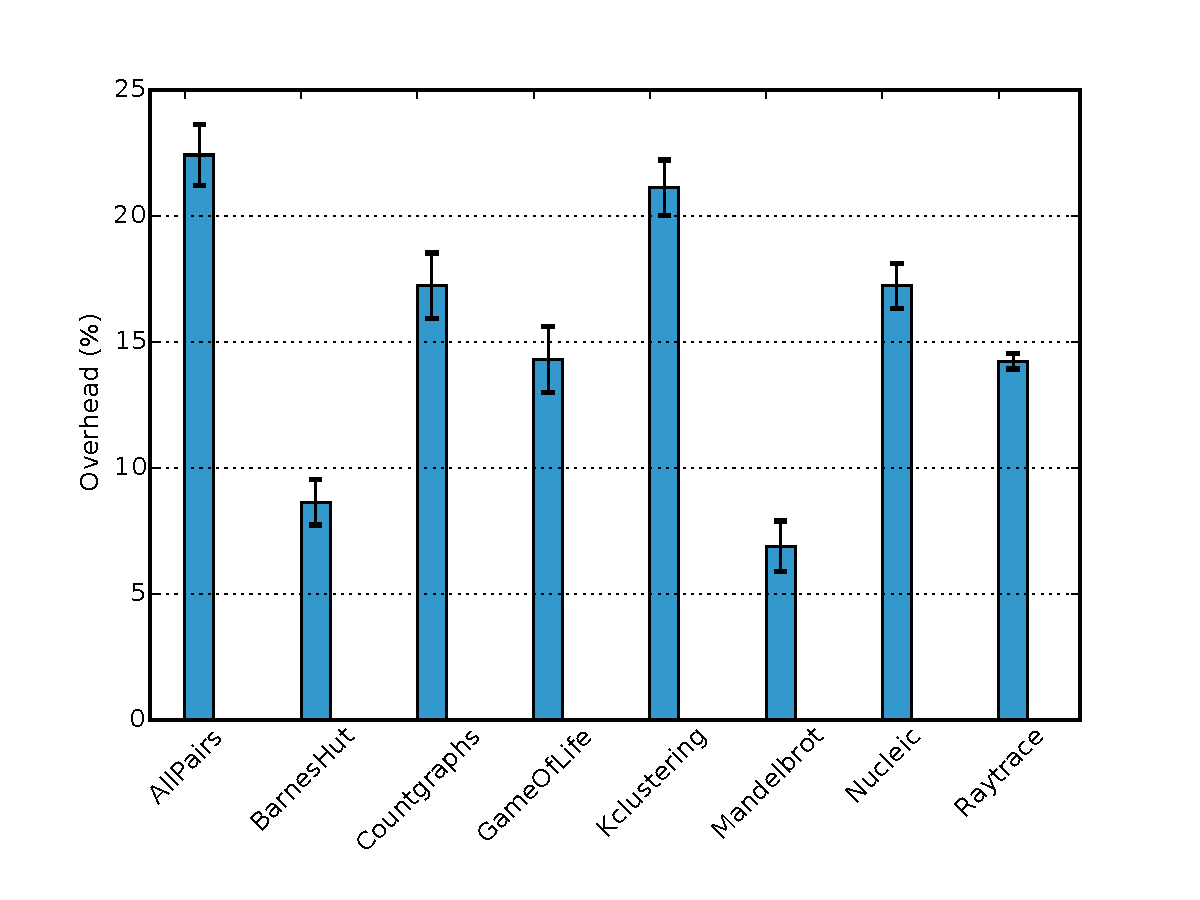
\includegraphics[width=0.9\textwidth]{Graphs/RB_overhead}
  \caption{Read barrier overhead as a percentage of mutator time.}
  \label{fig:rb-overhead}
\end{figure}

We evaluated a set of 8 benchmarks (described in Section~\ref{sec:gc_bench})
each running on all 48 cores on the SCC to measure read barrier overheads.
Figure~\ref{fig:rb-overhead} shows these overheads as a percentage of mutator
time. Our experiments reveal that, on average, the mutator spends 15.3\% of the
time executing read barriers for our benchmarks.

\begin{table}[hbt]
\begin{center}
\begin{tabular} {l r r}
\hline
{\bf Benchmark} & {\bf RB invocations ($\times 10^6$)} & {\bf Forwarded}\\
\hline
{AllPairs} & 9,753 & 123 \\
{BarnesHut} & 2,864 & 52,702 \\
{CountGraphs} & 2,584 & 0 \\
{GameOfLife} & 4,858 & 2,143 \\
{KClustering} & 3,780 & 101 \\
{Mandelbrot} & 2,980 & 23 \\
{Nucleic} & 2,887 & 328 \\
{Raytrace} & 2,217 & 0 \\
\hline
\end{tabular}
\end{center}
\caption{Effectiveness of read barrier checks: RB invocations represents the number of
read barrier invocations and forwarded represents the number of instances when
the read barrier encountered a forwarded object.}
\label{tab:rb_utility}
\end{table}

The next question to ask is whether the utility of the read barrier justifies
its cost. To answer this question, we measure the number of instances the read
barrier is invoked and the number of instances the barrier finds a forwarded
object (see Table~\ref{tab:rb_utility}).  We see that read barriers find
forwarded objects in less than one thousandth of a percent of the number of
instances they are invoked. Thus, in our system, the cost of read barriers is
substantial, but only rarely do they have to perform the task of forwarding
references. These results motivate our interest in a memory management design
that eliminates read barriers altogether.

\section{Procrastinating Collector Design}

Eliminating read barriers, however, is non-trivial. Abstractly, one can avoid
read barriers by eagerly \emph{fixing} all references that point to forwarded
objects at the time the object is lifted to the shared heap, ensuring the
mutator will never encounter a forwarded object. Unfortunately, this requires
being able to enumerate all the references that point to the lifted object; in
general, gathering this information is very expensive as the references to an
object might originate from any object in the local heap.

We consider an alternative design that completely eliminates the need for read
barriers \emph{without} requiring a full scan of the local heap whenever an
object is lifted to the shared heap.  The design is based on the observation
that read barriers can be clearly eliminated if forwarding pointers are never
introduced.  One way to avoid introducing forwarding pointers is to
\emph{delay} operations that create them until a local garbage collection is
triggered.  In other words, rather than executing a store operation that would
trigger lifting a thread local object to the shared heap, we can simply
\emph{procrastinate}, thereby stalling the thread that needs to perform the
store.  The garbage collector must simply be informed of the need to lift the
object's closure during its next local collection. After collection is
complete, the store can take place with the source object lifted, and all
extant heap references properly adjusted.  As long as there is sufficient
concurrency to utilize existing computational resources, in the form of
available runnable threads to run other computations, the cost of
procrastination is just proportional to the cost of a context switch.

Moreover, it is not necessary to always stall an operation that involves
lifting an object to the shared heap.  We consider a new property for objects
(and their transitive object closures) called \emph{cleanliness}.  A clean
object is one that can be safely lifted to the shared heap without introducing
forwarding pointers that might be subsequently encountered by the mutator:
objects that are immutable, objects only referenced from the stack, or objects
whose set of incoming heap references is known, are obvious examples.  The
runtime analysis for cleanliness is combined with a specialized write barrier
to amortize its cost.  Thus, procrastination provides a general technique to
eliminate read barriers, while cleanliness serves as an important optimization
that avoids stalling threads unnecessarily.

The effectiveness of our approach depends on a programming model in which (a)
most objects are clean, (b) the transitive closure of the object being lifted
rarely has pointers to it from other heap allocated objects, and (c) there is a
sufficient degree of concurrency in the form of runnable threads; this avoids
idling available cores whenever a thread is stalled performing an exporting
write that involves an unclean object.  We observe that conditions (a) and (b)
are common to functional programming languages and condition (c) follows from
the \acml\ runtime model. Our technique does not rely on programmer
annotations, static analysis or compiler optimizations to eliminate read
barriers, and can be completely implemented as a lightweight runtime technique.

